\section{Type Analyzer}\label{sec:analyzer}

In this section, we explain the detail of the type analyzer of $\tool$. We first
formally define a modified $\ires$ and explain how to perform type analysis for
the modified $\ires$.  Moreover, we also explain a condition-based refinement of
type analysis based on conditions of assertions and branches to increase
analysis precision.

\subsection{Intermediate Representation}\label{sec:ires}

\begin{figure}
  \centering
  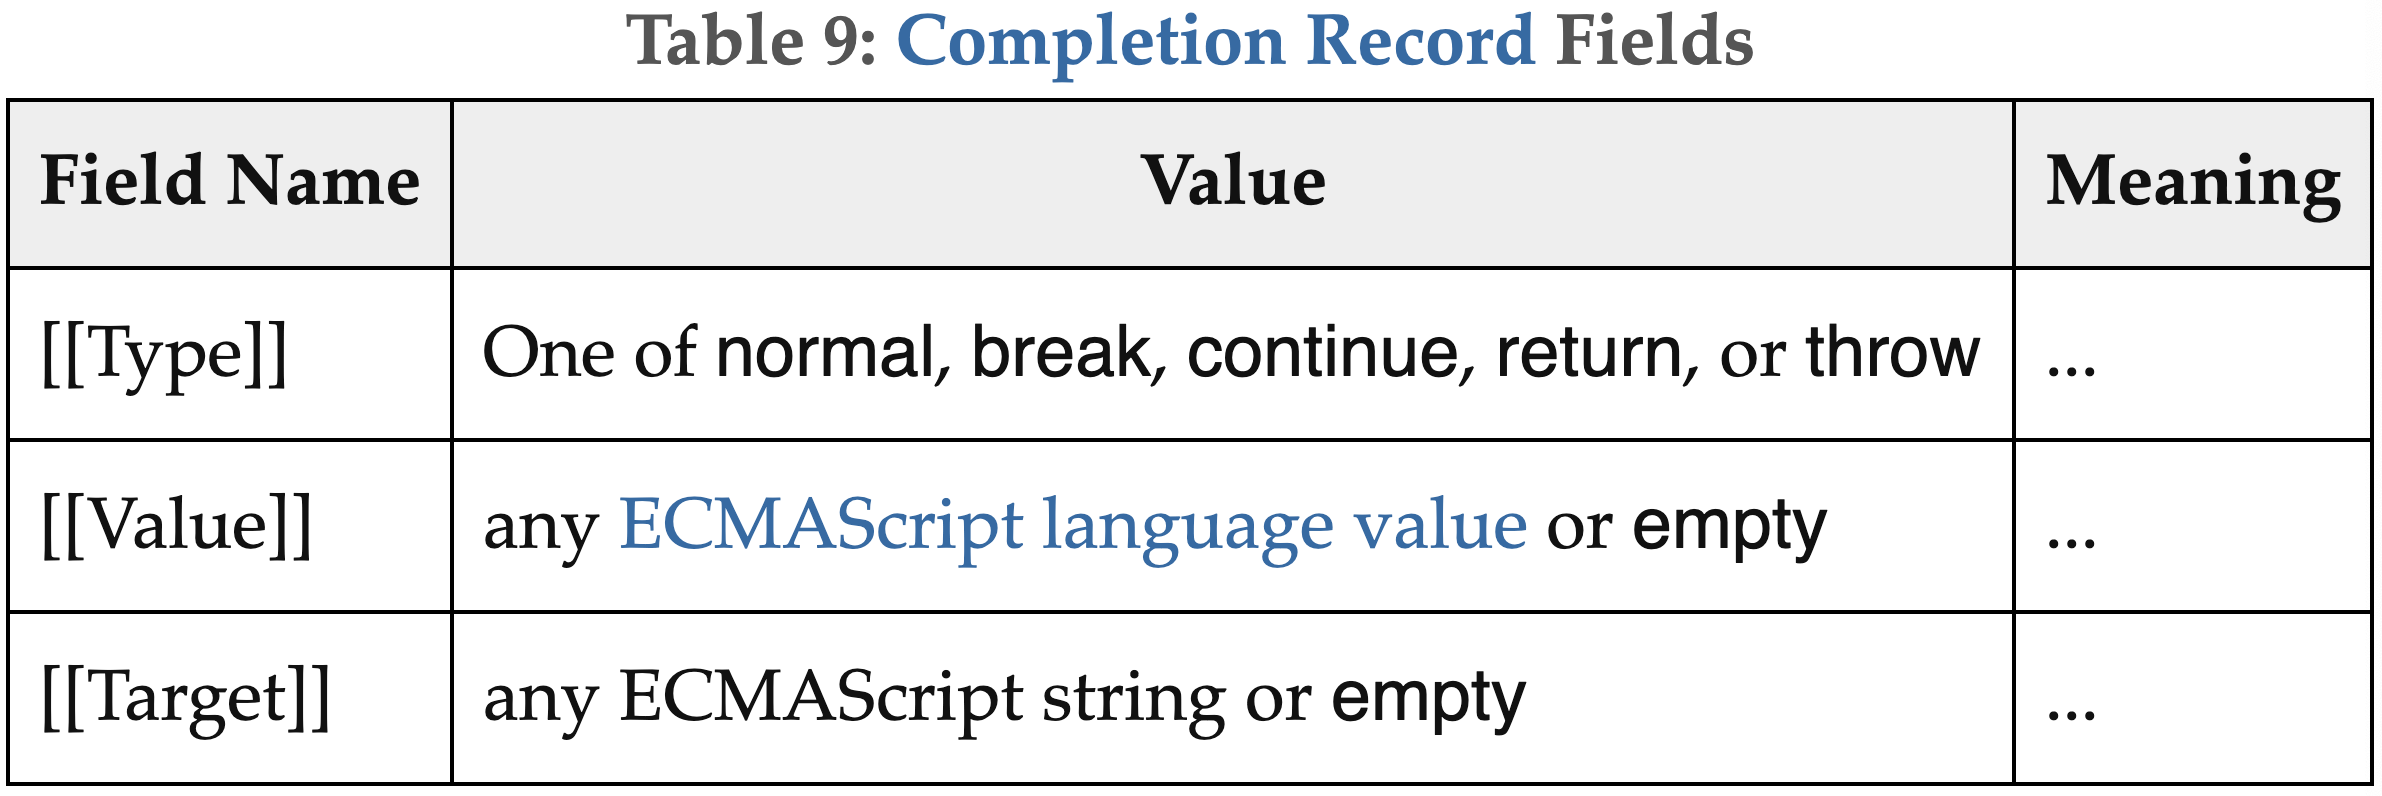
\includegraphics[width=0.48\textwidth]{img/record-fields-table}
  \vspace*{-1.5em}
  \caption{Fields of completion records in ES11.}
  \label{fig:record-fields-table}
  \vspace*{-1.5em}
\end{figure}

$\ires$ is an untyped intermediate representation introduced by \citet{jiset}.
To make it more suitable for type analysis, we modify it as a label-based
language as follows:
\small
\[
  \begin{array}{l@{~}r@{~}c@{~}r@{~}r@{~}l}
    \text{Functions}
    &\funcset&\ni&\func&::=&\kwdef \; \x (\x^*, \kwsl \x^* \kwsr). \; \lab\\

    \text{Instructions}
    &\instset&\ni&\inst&::=&
    \kwlet \; \x = \expr \mid
    \x = \kwrl \expr \; \expr^* \kwrr \mid
    \kwassert \; \expr \\

    &&&&\mid&
    \kwif \; \expr \; \lab \; \lab \mid
    \kwreturn \; \expr \mid
    \refer = \expr \\

    \text{References}
    &&&\refer&::=&
    \x \mid
    \refer \kwsl \expr \kwsr \\

    \text{Expressions}
    &&&\expr&::=&
    \tname \; \kwcl [\x: \expr]^* \kwcr \mid
    \clist{\expr^*} \mid
    \expr: \ty \mid
    \refer \kwexists \\

    &&&&\mid&
    \expr \bop \expr \mid
    \uop \; \expr \mid
    \refer \mid
    \const \mid
    \prim \\

    \text{Primitives}
    &\primset&\ni&\prim&::=&
    \undefval \mid \nullval \mid \bool \mid
    \num \mid \bigint \mid \str \mid \symb \\

    \text{Types}
    &\tyset&\ni&\ty&::=&\tname \mid \clist{} \mid \clist{\ty} \mid \tjs \mid
    \tprim \mid \undefval \mid \nullval\\

    &&&&\mid&
    \tbool \mid \tnumeric \mid \tnum \mid \tbigint \mid \tstr \mid \tsymb \\
  \end{array}
\]

A modified $\ires$ program $\prog = (\getfunc, \getinst, \getnext)$ is consists
of three mappings from labels;  $\getfunc: \labset \rightarrow \funcset$
represents that labels are in which functions, $\getinst: \labset \rightarrow
\instset$ represents instructions attached to labels, and $\getnext: \labset
\rightarrow \labset$ denotes next labels where a label $\lab \in \labset$
denotes a program point.  function $\kwdef \; \f (\x^*, \kwsl \y^* \kwsr). \;
\lab \in \funcset$ consists of its name $\f$, normal parameters $\x^*$, optional
parameters $\y^*$, and a body label $\lab$.  Although global variables exist in
ECMAScript, we assume that only local variables exist in this paper for brevity
An instruction $\inst$ is a variable declaration, a function call, an assertion,
a branch, a return, or an reference update.  Each invocation of an abstract
algorithm in ECMAScript is compiled to a function call instruction with a newly
introduced temporal variable.  We represent loops using branch instructions with
cyclic pointing of labels in the next mapping $\getnext$.  A reference $\refer$
is a variable $\x$ or a field access $\refer \kwsl \expr \kwsr$.  We use the
notation $\refer.\f$ to briefly represent $\refer \kwsl \code{"f"} \kwsr$. An
expression $\expr$ is a record, a list, a type check, an existence check, a
binary operation, a unary operation, a reference, a constant, or a primitive,
which is either $\undefval$, $\nullval$, a Boolean $\bool$, a Number $\num$, a
BigInt $\bigint$, a String $\str$, or a Symbol $\symb$.

\begin{figure}
  \centering
  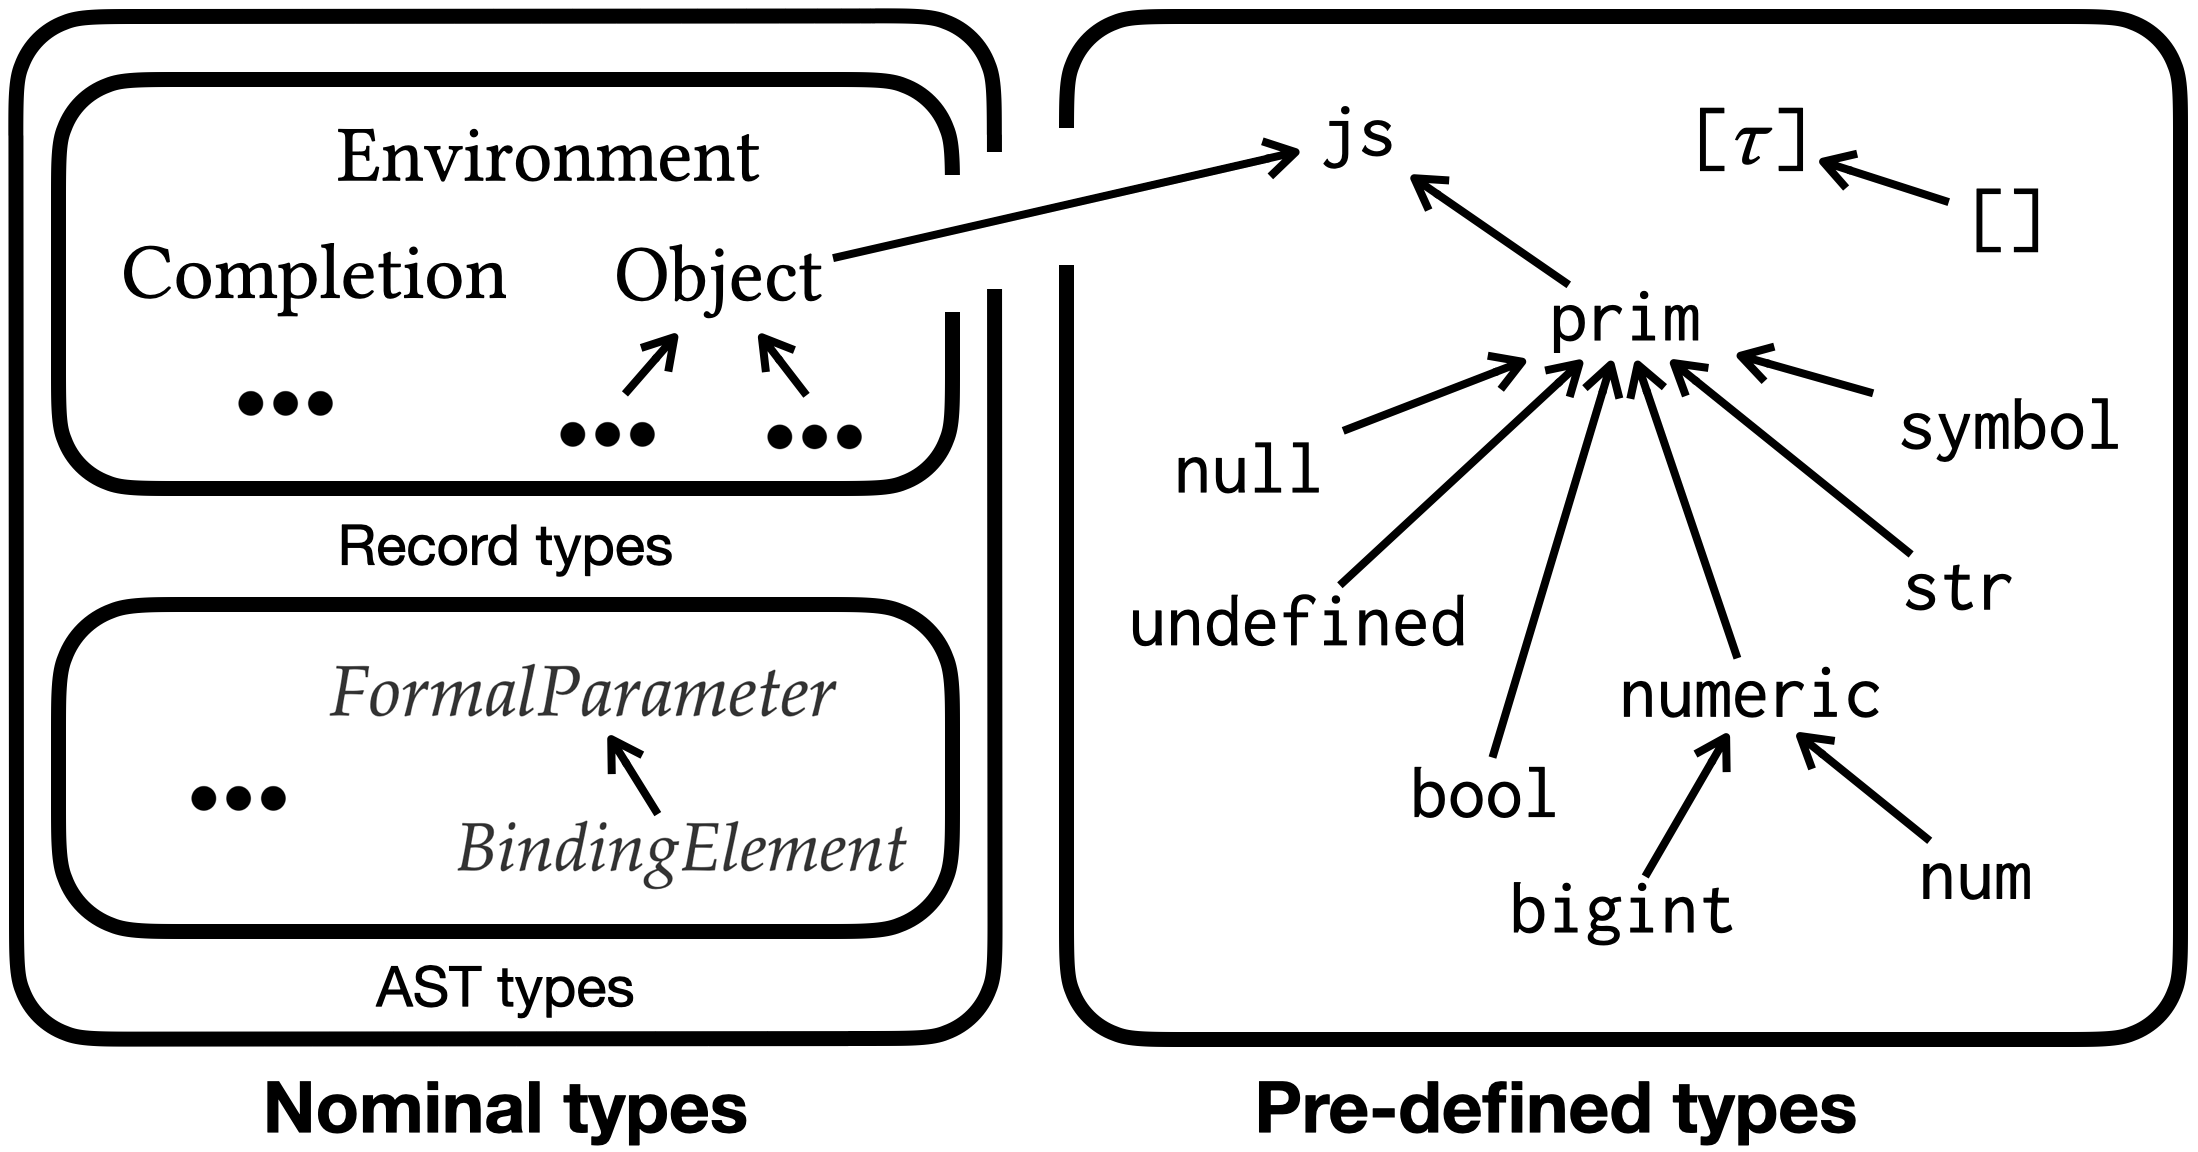
\includegraphics[width=0.4\textwidth]{img/subtype}
  \vspace*{-1.5em}
  \caption{A graphical representation of subtype relation $\subtype$.}
  \label{fig:subtype}
  \vspace*{-1.5em}
\end{figure}

A type $\ty \in \tyset$ is a norminal type $\tname$ or a pre-defined type;
$\tjs$ denotes JavaScript values, $\tprim$ primitives, $\tnumeric$ either Number
or BigInt values, and $\tnum$, $\tbigint$, $\tstr$, and $\tsymb$ denote Number,
BigInt, String, and Symbol values, respectively.  A norminal type $\tname$ is
either 1) a \textit{production type} for ASTs or 2) a \textit{record type} used
in abstract algorithms, and ECMAScript describes its fields with pre-defined or
possible values.  A production type has corresponding syntax-directed algorithms
as its fields and a record type has specific fields with possible values
described in the corresponding table and additional description in ECMAScript.
The production type is automatically extracted but we manually model fields of
record types.  For example, Figure~\label{fig:record-fields-table} is an excerpt
from ES11 that describes fields of completion
records~\footnote{https://262.ecma-international.org/11.0/\#table-8}; it
contains three fields ``Type'' with a constant such as \code{normal}, ``Value''
with JavaScript values or an constant \code{empty}, and ``Target'' with String
values or \code{empty}.  We manually model them as follows:
\small
\[
  \begin{array}{l}
    \text{Completion} = \kwcl\\
    \quad \Type: \kwcl \nconst{normal}, \nconst{break}, \nconst{continue},
    \nconst{return}, \nconst{throw} \kwcr\\
    \quad \Value: \kwcl \tjs, \nconst{empty} \kwcr\\
    \quad \Target: \kwcl \tstr, \nconst{empty} \kwcr\\
    \kwcr\\
  \end{array}
\]

The subtype relation $\subtype \subseteq \tyset \times \tyset$ between types is
depicted in Figure~\ref{fig:subtype}; the directed edge from $\ty'$ to $\ty$
denotes $\ty' \subtype \ty$ and the relation is reflexive and transitive.  The
subtype relation is dependent on the syntax and defined record types in
ECMAScript.  We extract subtypes for production types and manually model
subtypes between record types.  For example, consider the syntax-directed
abstract algorithm at the lower-right in Figure~\ref{fig:example}.  The
non-terminal \textit{BindingElement} is the unique token in a alternative of
\textit{FormalParameter} production thus we automatically extract the subtype
relation: \textit{BindingElement} $\subtype$ \textit{FormalParameter}.  Based on
this subtype relation, a type check expression $\expr: \ty$ checks whether the
evaluation result of $\expr$ has a type $\ty'$ satisfying $\ty' \subtype \ty$.

We define a denotational semantics of the modified $\ires$ for instructions
$\semi{\inst}: \dom \rightarrow \dom$, references $\semr{\refer}: \dom
\rightarrow \valset$, and expressions $\seme{\expr}: \dom \rightarrow \valset$.
For presentation brevity, we omit it in this paper and include it in a companion
report~\inred{\cite{report}}.


\subsection{Type Analysis}\label{sec:analysis}

\begin{figure*}[t]
  \centering
  \begin{subfigure}[b]{\textwidth}
    \[
      \begin{array}{r@{~}c@{~}ll}
        \asemi{\kwlet \; \x = \expr}
        (\lab, \tys)(\aelem) &=&
        (\{ (\getnext(\lab), \tys) \mapsto \aenv_\x \}, \emp) &
        \text{where} \;
        \aenv_\x = \aenv[\x \mapsto \aty] \wedge
        \aty = \aseme{\expr}(\aenv)\\

        \asemi{\x = \kwrl \expr_0 \; \expr_1 \cdots \expr_n \kwrr}
        (\lab, \tys)(\aelem) &=&
        \left(
          \begin{array}{@{}l@{}}
            \{ (\lab_\func, \tys_a) \mapsto \aenv_{\func, \tys_a} \mid \func \in
              F \wedge \tys_a \in T_a
            \},\\
            \{ (\func, \tys_a) \mapsto \{ (\getnext(\lab), \tys, \x) \} \mid
              \func \in F \wedge \tys_a \in T_a
            \}\\
          \end{array}
        \right) &
        \text{where} \;
        \left\{
          \begin{array}{@{}l@{}}
            \aty_i = \aseme{\expr_i}(\aenv) \wedge T_a = \{ \upcasts([ \ty_1,
            \cdots, \ty_n ] \mid \ty_i \in \aty_i \} \wedge\\
            F = \{ \func \in \aty_0 \mid \func = \kwdef \; \_ (\p_1, \cdots,
            \kwsl \cdots, \p_m \kwsr). \; \lab_\func \} \wedge\\
            \aenv_{\func, \tys_a} = \aenv[\p_1 \mapsto \{ \tys_a[1] \}, \cdots,
            \p_m \mapsto \{ \tys_a[m] \}]\\
          \end{array}
        \right.\\

        \asemi{\kwassert \; \expr}
        (\lab, \tys)(\aelem) &=&
        (\{ (\getnext(\lab), \tys) \mapsto \aenv_\mt \}, \emp) &
        \text{where} \; \aenv_\mt = \refine(\expr, \true)(\aenv)\\

        \asemi{\kwif \; \expr \; \lab_\mt \; \lab_\mf}
        (\lab, \tys)(\aelem) &=&
        (\{ (\lab_\mt, \tys) \mapsto \aenv_\mt, (\lab_\mf, \tys) \mapsto
        \aenv_\mf \}, \emp) &
        \text{where} \;
        \aenv_\mt = \refine(\expr, \true)(\aenv) \wedge
        \aenv_\mf = \refine(\expr, \false)(\aenv)\\

        \asemi{\kwreturn \; \expr}
        (\lab, \tys)(\aelem) &=&
        (\{ (\lab_r, \tys_r) \mapsto \aenv_r \mid (\lab_r, \tys_r, \x) \in
        \retp(\getfunc(\lab), \tys)\}, \emp) &
        \text{where} \;
        \aelem = (\rmap, \retp) \wedge
        \aenv_r = \rmap(\lab_r, \tys_r)[\x \mapsto \aty] \wedge
        \aty = \aseme{\expr}(\aenv)\\

        \asemi{\x = \expr}
        (\lab, \tys)(\aelem) &=&
        (\{ (\getnext(\lab), \tys) \mapsto \aenv_\x \}, \emp) &
        \text{where} \;
        \aenv_\x = \aenv[\x \mapsto \aty] \wedge
        \aty = \aseme{\expr}(\aenv)\\

        \asemi{\refer \kwsl \expr_0 \kwsr = \expr_1}
        (\lab, \tys)(\aelem) &=&
        (\{ (\getnext(\lab), \tys) \mapsto \aenv \}, \emp)
      \end{array}
    \]
    \caption{Instructions with $\asemi{\inst}: (\labset \times \tyset^*)
    \rightarrow \adom \rightarrow \adom$ where $\aenv = \aelem(\lab, \tys)$.}
  \end{subfigure}
  \begin{subfigure}[b]{0.48\textwidth}
    \[
      \asemr{\x}(\aenv) = \aenv(\x)
      \qquad
      \asemr{\refer \kwsl \expr \kwsr}(\aenv) = \{ \ty[\str] \mid \ty \in
      \asemr{\refer}(\aenv) \wedge \str \in \aseme{\expr}(\aenv) \}
    \]
    \caption{References with $\asemr{\refer}: \aenvset \rightarrow \atyset$.}
  \end{subfigure}
  \begin{subfigure}[b]{\textwidth}
    \[
      \begin{array}{r@{~}c@{~}lr@{~}c@{~}lr@{~}c@{~}l}
        \aseme{\tname \; \kwcl \fields \kwcr}(\aenv)
        &=& \multicolumn{7}{@{}l}{
          \left\{
            \begin{array}{ll}
              \{ \tnormal(\ty) \mid \ty \in \aseme{\fields(\code{Value})}(\aenv)
              \} & \text{if} \; \tname = \text{Completion} \wedge
              \fields(\code{Type}) = \nconst{normal}\\

              \{ \tabrupt \} & \text{if} \; \tname = \text{Completion} \wedge
              \fields(\code{Type}) \neq \nconst{normal}\\

              \{ \tname \} & \text{otherwise}\\
            \end{array}
          \right.
          \quad \aseme{\prim}(\aenv) =
          \left\{
            \begin{array}{ll}
              \{ \tnum \} & \text{if} \; \prim = \num\\
              \{ \tbigint \} & \text{if} \; \prim = \bigint\\
              \{ \tsymb \} & \text{if} \; \prim = \symb\\
              \{ \prim \} & \text{otherwise}\\
            \end{array}
          \right.
        }

        \\

        \aseme{\const}(\aenv) &=& \const &

        \aseme{\clist{}}(\aenv) &=& \clist{} &

        \aseme{\clist{\expr_0, \cdots, \expr_n}}(\aenv)
        &=& \{ \clist{\ty} \mid \ty \in \bigjoin_{0 \leq i
        \leq n} \aseme{\expr_i}(\aenv) \}

        \\

        \aseme{\expr: \ty}(\aenv)
        &=& \{ \ty' \subtype \ty \mid \ty' \in
        \aseme{\expr}(\aenv) \} &

        \aseme{\refer \kwexists}(\aenv)
        &=& \{ \ty \neq \tabsent \mid \ty \in
        \aseme{\expr}(\aenv) \} &

        \aseme{\refer}(\aenv)
        &=& \asemr{\refer}(\aenv) \setminus \{ \tabsent \}

        \\

        \aseme{\uop \; \expr}(\aenv)
        &=& \{ \abs{\uop} \ty \mid \ty \in
        \aseme{\expr}(\aenv) \} &

        \aseme{\expr_0 \bop \expr_1}(\aenv)
        &=& \multicolumn{4}{@{}l}{\{ \ty_0 \abs{\bop} \ty_1 \mid \ty_0 \in
        \aseme{\expr_0}(\aenv) \wedge \ty_1 \in \aseme{\expr_1}(\aenv) \}}

        \\
      \end{array}
    \]
    \caption{Expressions with $\aseme{\expr}: \aenvset \rightarrow \atyset$.}
  \end{subfigure}
  \caption{Abstract semantics of the modified $\ires$ for a program $\prog =
  (\getfunc, \getinst, \getnext)$.}
  \vspace*{-1.5em}
  \label{fig:abs-sem}
\end{figure*}

We design a type analysis for the modified $\ires$ based on abstract
interpretation framework~\cite{ai1977, ai1992} with analysis
sensitivity~\cite{sens-toplas}.  We first extend types $\tyset$ as follows:
\[
  \tyset \ni \ty ::=
  \cdots \mid
  \func \mid
  \const \mid
  \tnormal(\ty) \mid
  \tabrupt \mid
  \bool \mid
  \str \mid
  \tabsent
\]
There are three different reasons why we extend types.  First, the original
types $\tyset$ do not cover all types of values thus we add functions and
constants.  Second, we add more specific types to increase the precision of type
analysis.  A completion record is a \textit{normal completion} when its Type
field is a constant $\nconst{normal}$ or an \textit{abrupt completion}
otherwise.  We add $\tnormal(\ty)$ and $\tabrupt$ for normal and abrupt
completions.  Moreover, we also add Boolean values $\bool$, and String values
$\str$ to precisely handle the control flows of branches and field accesses,
respectively.  Third, we add the absent type $\tabsent$ to represent the
existence of variables.  Using such extended types, we define abstract states
with flow-sensitivity and type-sensitivity for parameters:
\[
  \begin{array}{lr@{~}c@{~}c@{~}r@{~}l}
    \text{Abstract States}
    &\aelem&\in&\adom&=& \rmapset \times \retpset\\

    \text{Result Maps}
    &\rmap&\in&\rmapset&=& \labset \times \tyset^* \rightarrow \aenvset\\

    \text{Return Points}
    &\retp&\in&\retpset&=& \funcset \times \tyset^*
    \rightarrow \partsof{\labset \times \tyset^* \times \varset} \\

    \text{Abstract Environments}
    &\aenv&\in&\aenvset&=&\varset \rightarrow \atyset\\

    \text{Abstract Types}
    &\aty&\in&\atyset&=&\partsof{\tyset}\\
  \end{array}
\]
An abstract state $\aelem \in \adom$ is pair of a return map and a return point
mapping.  A result map $\rmap \in \rmapset$ represents an abstract environment
for each flow-sensitive and type-sensitive view, and a return point mapping
$\retp \in \retpset$ represents possible return points of each function with
a type-sensitive context.  An abstract environment $\aenv \in \aenvset$
represents possible types of each variable, and $\aenv(\x) = \{ \tabsent \}$
when $\x$ is not defined in $\aenv$.  An abstract type $\aty \in \atyset$ is a
set of types.  While we define the join operator $\join$, the meet operator
$\meet$, and the partial order $\order$ for most of abstract domains in a
point-wise manner, we define the operators for types with a normalization
function $\norm$ because of their subtype relations:
\[
  \begin{array}{l}
    \aty_0 \join \aty_1 = \norm(\aty_0 \cup \aty_1)\\
    \aty_0 \meet \aty_1 = \norm(
      \{\ty_0 \in \aty_0 \mid \{ \ty_0 \} \order \aty_1 \} \cup
      \{\ty_1 \in \aty_1 \mid \{ \ty_1 \} \order \aty_0 \}
    )\\
    \aty_0 \order \aty_1 \Leftrightarrow \forall \ty_0 \in \aty_0. \; \exists
    \ty_1 \in \norm(\aty_1). \; \text{s.t.} \; \ty_0 \subtype \ty_1\\
  \end{array}
\]
where $\norm(\aty) = \{ \ty \mid \ty \in \aty_e \wedge \not\exists \ty' \in
\aty_e. \; \text{s.t.} \; \ty \neq \ty' \wedge \ty \subtype \ty' \}$.

Based on abstract states, we define the abstract semantics of instructions,
references, and expressions in the modified $\ires$ described in
Figure~\ref{fig:abs-sem}.  To prevent the explosion of the number of type-sensitive
views, we upcast the type of each argument before function calls with the
following function:
\[
  \upcast(\ty) = \left\{
    \begin{array}{ll}
      \tnormal(\upcast(\ty')) & \text{if} \; \ty = \tnormal(\ty')\\
      \clist{\upcast(\ty')} & \text{if} \; \ty = \clist{\ty'}\\
      \tstr & \text{if} \; \ty = \str\\
      \tbool & \text{if} \; \ty = \bool\\
      \ty & \text{otherwise}\\
    \end{array}
  \right.
\]
and $\upcasts$ denotes a point-wise extension of $\upcast$ for type sequences.
For branches and assertions, we apply the $\refine$ function that prunes out
infeasible parts in abstract environments based on their conditions to increase
analysis precision.  We explain its detail in Section~\ref{sec:refine}.  Then,
we define the abstract semantics $\asem{\prog}$ of a program $\prog = (\getfunc,
\getinst, \getnext)$ as the least fixpoint of abstract transfer $\atransfer:
\adom \rightarrow \adom$:
\[
  \begin{array}{r@{~}c@{~}l}
    \asem{\prog} &=& \lim_{n \rightarrow \infty}(\atransfer)^n(\iaelem)\\
    \atransfer(\aelem) &=& \aelem \join \left(
      \underset{(\lab, \tys) \in \domain{\rmap}}{\bigjoin}
      \asemi{\getinst(\lab)}(\lab, \tys)(\aelem)
    \right)\\
  \end{array}
\]
where $\aelem = (\rmap, \_)$ and $\iaelem$ denotes the initial abstract state.
As described in the Section~\ref{sec:overview}, $\iaelem$ contains all
syntax-directed algorithms having no additional parameters and built-in
algorithms with appropriate abstract environments.  For syntax-directed
algorithms, we construct its abstract environment containing the variable
$\this$ with a production type and other variables for non-terminals.  For
example, the upper-left syntax-directed algorithm in Figure~\ref{fig:example} is
initialized with the following abstract environment:
\[
  \left\{
    \begin{array}{r@{~}c@{~}l}
      \this &\mapsto& \{ \text{AssignmentExpression} \},\\
      \mcode{LeftHandSideExpression} &\mapsto& \{ \text{LeftHandSideExpression} \},\\
      \mcode{AssignmentExpression} &\mapsto& \{ \text{AssignmentExpression} \}
    \end{array}
  \right.
\]
For built-in algorithms, we assign pre-defined variables $\this$, $\args$, and
$\NewTarget$ with corresponding types and parameters with $\tjs$ types.  For
example, the following abstract environment is for the built-in
algorithm $\jscode{Math.round}$ at the upper-right in Figure~\ref{fig:example}:
\[
  \left\{
    \begin{array}{r@{~}c@{~}l}
      \this &\mapsto& \{ \tjs \},
      \args \mapsto \{ \clist{\tjs} \},
      \x \mapsto \tjs\\
      \NewTarget &\mapsto& \{ \text{Object}, \undefval \},\\
    \end{array}
  \right.
\]


\subsection{Condition-based Refinement}\label{sec:refine}

We present a \textit{condition-based refinement} of type analysis for the
modified $\ires$ to increase analysis precision.  It prunes out infeasible parts
in abstract environments based on conditions of branches of assertions, and we
formally define the $\refine$ function as a composition of two functions
$\refineFlow$ and $\refineVar$:
\[
  \refine(\expr, \bool) =
  \refineVar(\expr, \bool) \circ \refineFlow(\expr, \bool)
\]
The $\refineFlow$ prevents infeasible \textit{control flows} by producing an
empty abstract environment as follows:
\[
  \refineFlow(\expr, \bool)(\aenv) = \left\{
    \begin{array}{ll}
      \aenv & \text{if} \; \{ \bool \} \order \aseme{\expr}(\aenv)\\
      \emp & \text{otherwise}\\
    \end{array}
  \right.
\]
Beyond control flows, $\refineVar$ refines the shape of a given abstract
environment based on the conditions for variables:
\[
  \begin{array}{r@{~}c@{~}l}
    \refineVar(\code{!} \expr, \bool)(\aenv) &=&
    \refineVar(\expr, \neg \bool)(\aenv)\\

    \refineVar(\expr_0 \bop \expr_1, \bool)(\aenv) &=&
    \left\{
      \begin{array}{ll}
        \aenv_0 \join \aenv_1 & \text{if} \; \bool \wedge \bop = \code{||}\\
        \aenv_0 \meet \aenv_1 & \text{if} \; \neg\bool \wedge \bop = \code{||}\\
        \aenv_0 \meet \aenv_1 & \text{if} \; \bool \wedge \bop = \code{\&\&}\\
        \aenv_0 \join \aenv_1 & \text{if} \; \neg\bool \wedge \bop = \code{\&\&}\\
        \aenv & \text{otherwise}\\
      \end{array}
    \right.\\
    \multicolumn{3}{r}{
      \text{where} \;
      \aenv_0 = \refineVar(\expr_0, \bool)(\aenv) \wedge
      \aenv_1 = \refineVar(\expr_1, \bool)(\aenv)
    }\\

    \refineVar(\x.\Type \code{=} \nconst{normal}, \true)(\aenv) &=&
    \aenv[ \x \mapsto \aseme{\x}(\aenv) \cap \tnormal(\tyset) ]\\
    \refineVar(\x.\Type \code{=} \nconst{normal}, \false)(\aenv) &=&
    \aenv[ \x \mapsto \aseme{\x}(\aenv) \cap \{ \tabrupt \} ]\\

    \refineVar(\x \code{=} \expr, \true)(\aenv) &=&
    \aenv[ \x \mapsto \aseme{\x}(\aenv) \meet \aseme{\expr}(\aenv) ]\\
    \refineVar(\x \code{=} \expr, \false)(\aenv) &=&
    \aenv[ \x \mapsto \aseme{\x}(\aenv) \setminus
    \lfloor\aseme{\expr}(\aenv)\rfloor ]\\

    \refineVar(\x : \ty, \true)(\aenv) &=&
    \aenv[ \x \mapsto \aseme{\x}(\aenv) \meet \{ \ty \} ]\\
    \refineVar(\x : \ty, \false)(\aenv) &=&
    \aenv[ \x \mapsto \aseme{\x}(\aenv) \setminus \{ \ty' \mid \ty' \subtype \ty
    \}]\\
  \end{array}
\]
and it returns $\aenvset$ for other cases.  The notation $\getSingle{\aty}$ denotes
to checks whether it is a singleton; $\getSingle{\aty} = \aty$ if $\aty = \{ \ty
\}$ and $\ty$ is a singleton type such as a constant $\const$, an empty list
$\clist{}$, an absent value $\tabsent$, a primitive value, etc., and
$\getSingle{\aty} = \emp$ otherwise.
